\documentclass{article}

\usepackage[education, final]{neurips_2026}

\usepackage[utf8]{inputenc}
\usepackage[T1]{fontenc}
\usepackage{hyperref}
\usepackage{url}
\usepackage{booktabs}
\usepackage{amsmath}
\usepackage{xcolor}
\usepackage{graphicx}

\title{Is Speculative Decoding All We Need?\\ A Visual Walkthrough from Autoregressive Decoding to Confidence-Scheduled Drafting}

\author{%
  Lily Zhang \\
  \texttt{@lily\_gpupoor} \\
}

\begin{document}

\maketitle

\begin{abstract}
A single-poster, plain-language walkthrough of speculative decoding for LLM inference, built as a four-stage progression: vanilla autoregressive decoding, EAGLE-3 draft-and-verify, DFlash block-parallel drafting, and DSpark confidence-scheduled trimming. It translates a systems technique into user-facing intuition (``fewer seconds staring at the terminal'') and ends on an honest, unresolved question: the base method is provably lossless, but the frontier tricks that push speed further trade a little exactness on the long tail, and almost nobody measures it. It was stress-tested at the AI Engineer conference, where repeated requests for a walkthrough motivated this submission.
\end{abstract}

\section{Concept Summary}
Autoregressive LLM decoding is \emph{memory-bandwidth bound}, not compute bound: generating one token streams the entire weight matrix from HBM while most compute units sit idle. A forward pass over $K$ tokens costs almost the same wall-clock time as a pass over one, so \emph{verifying} many tokens at once is nearly free. Speculative decoding exploits this: a small draft model proposes $K$ tokens, and the target model verifies all $K$ in a single pass, accepting a correct prefix via rejection sampling so the output distribution matches the target exactly.

Figure~\ref{fig:walkthrough} walks the four-stage story, each stage removing the previous bottleneck (tokens per target-model pass; Qwen3-4B code average, DSpark Table~1): \textbf{Vanilla} (1/pass) $\to$ \textbf{EAGLE-3} ($\sim$3.9) $\to$ \textbf{DFlash} ($\sim$4.4, block-parallel draft) $\to$ \textbf{DSpark} ($\sim$5.1, sequential head $+$ confidence-scheduled trimming). The ``aha'': \emph{we did not make the big model faster; we made it open fewer times.} The title's honest answer is \emph{no} --- the base method is lossless, but confidence-scheduled trimming and FP8 quantization slide toward lossy on the long tail, and almost nobody measures it.

\begin{figure}[t]
  \centering
  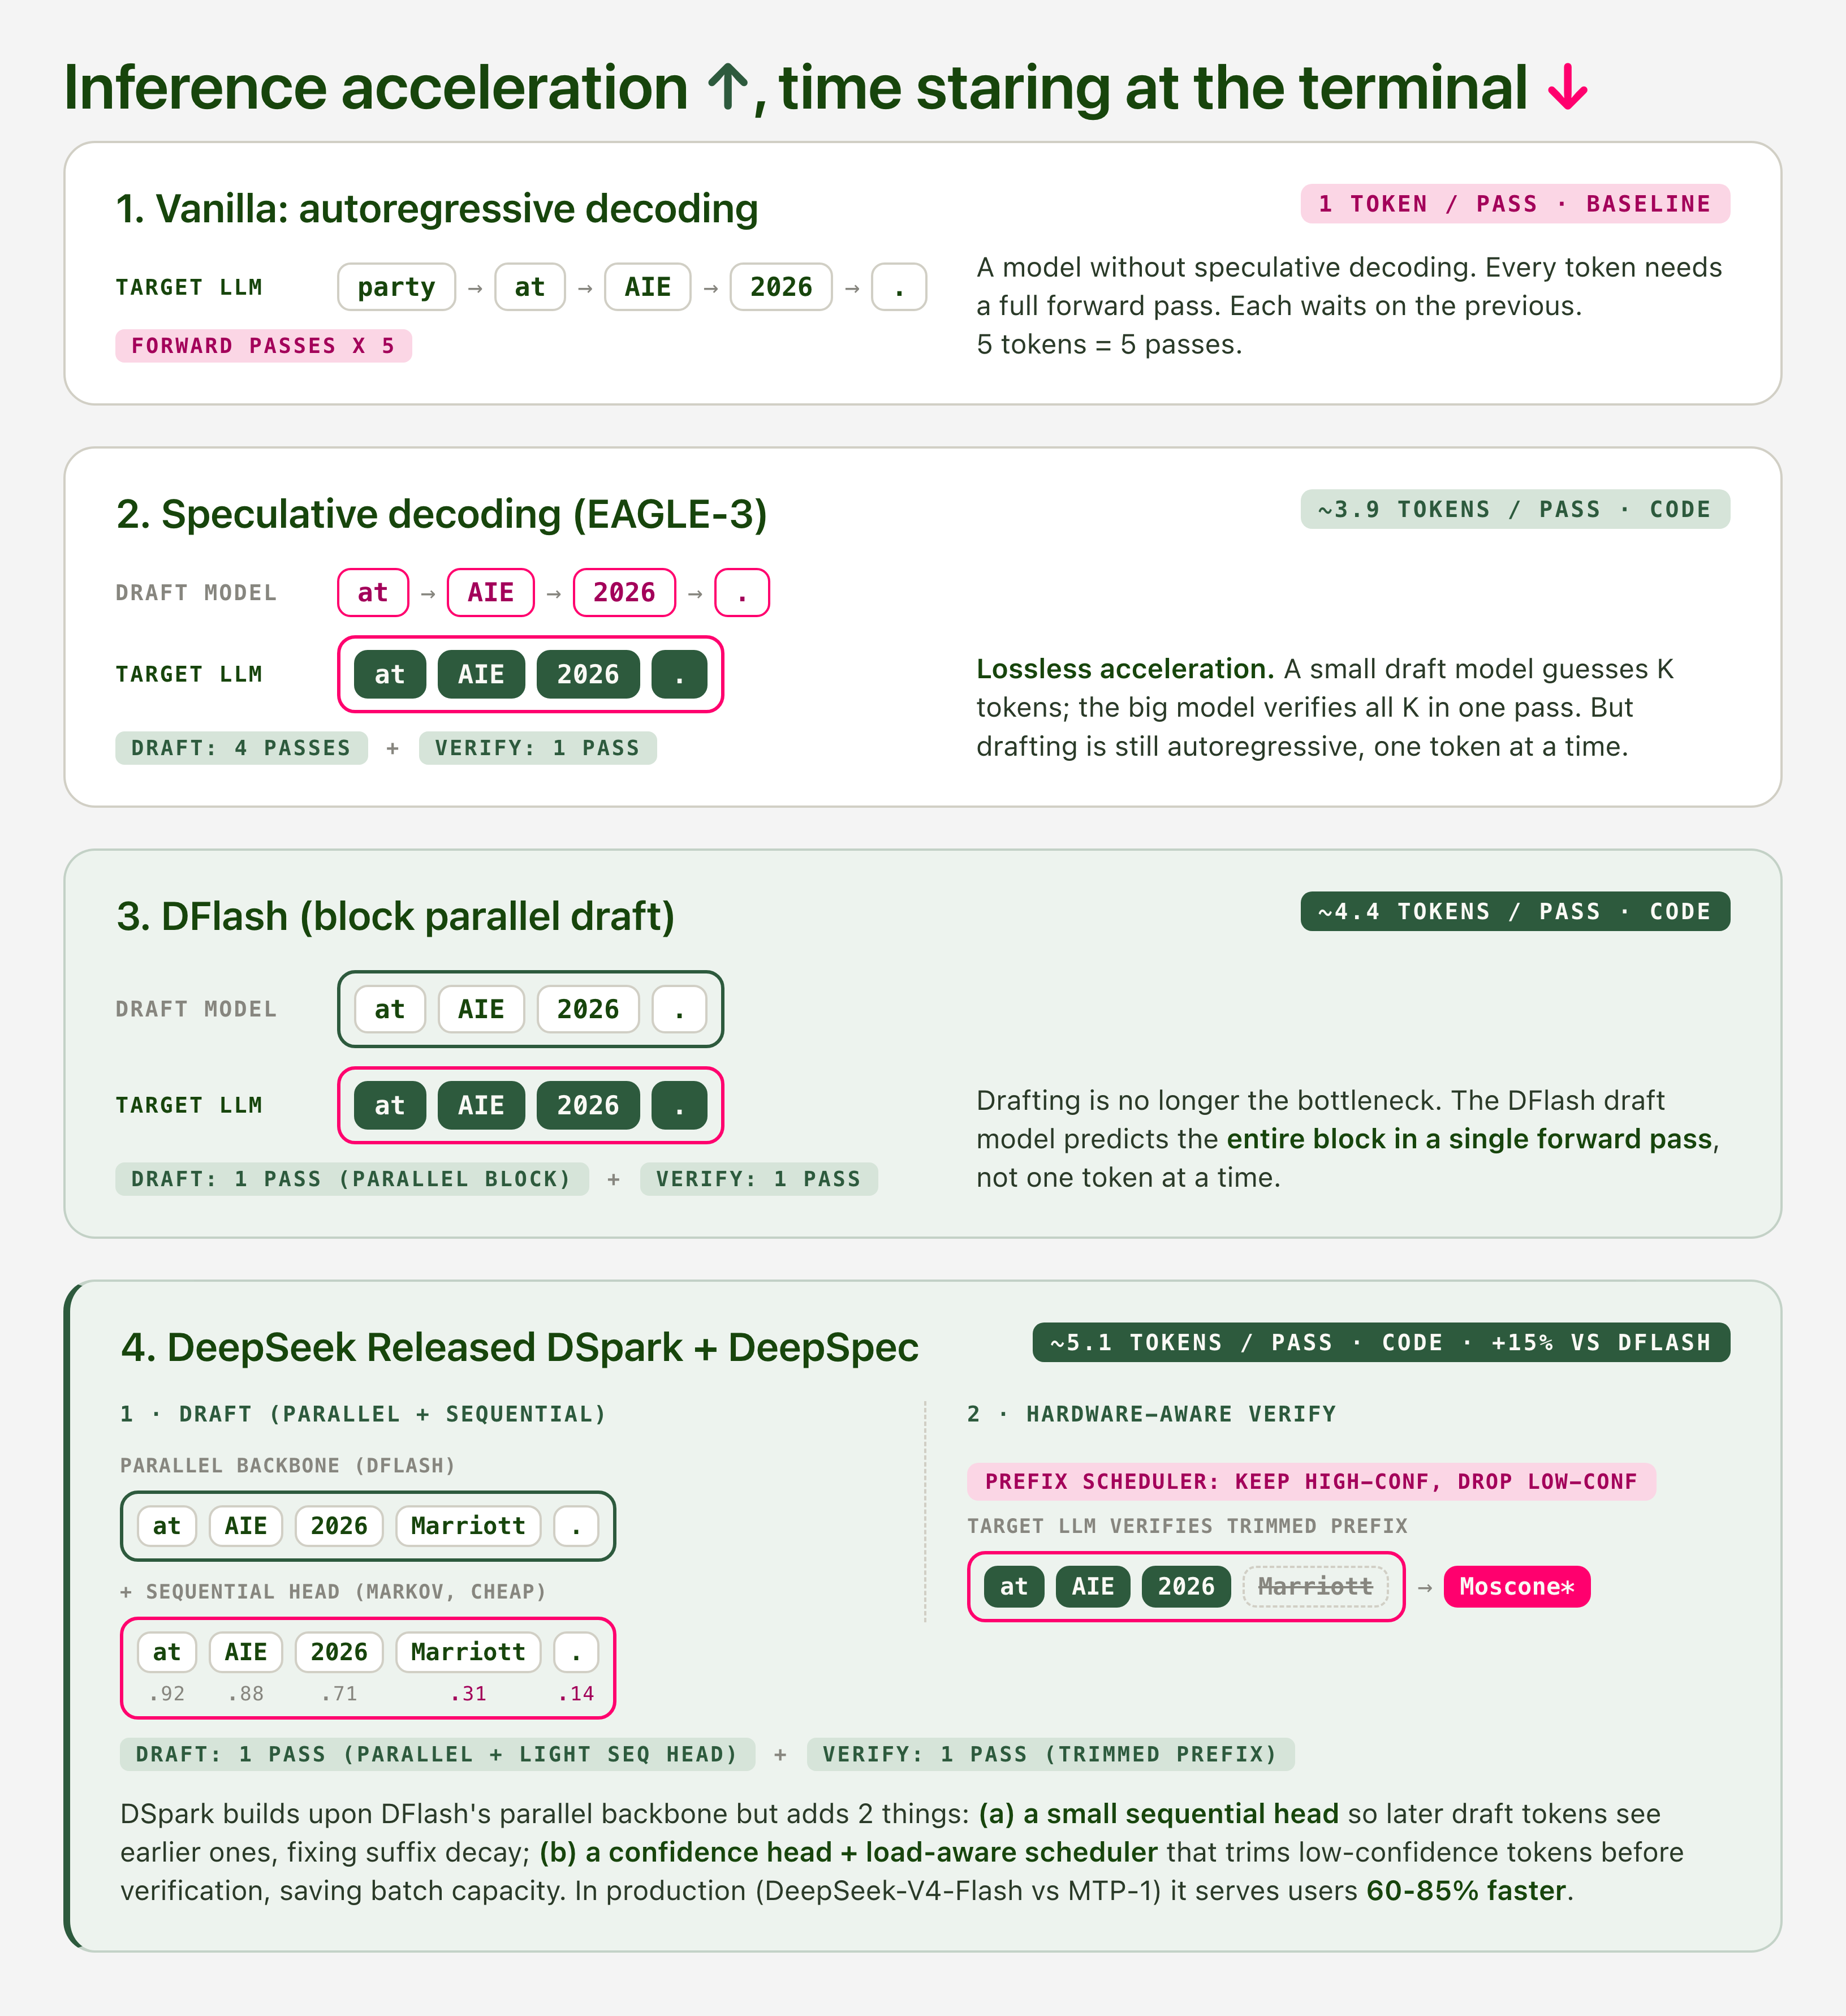
\includegraphics[width=0.46\textwidth]{../figures/figure-walkthrough.png}
  \caption{The core teaching visual: one worked example (``\texttt{at AIE 2026 .}'') carried across all four stages, with tokens-per-pass and accept/reject mechanics shown in place. The DSpark panel makes the lossless-vs-lossy boundary concrete: a low-confidence draft (``Marriott,'' 0.31) is trimmed before verification and corrected to ``Moscone.''}
  \label{fig:walkthrough}
\end{figure}

\section{Prerequisites and Technical Level}
\textbf{Level:} accessible to any engineer or student who knows that an LLM generates text one token at a time. \textbf{Prerequisites:} basic familiarity with transformer inference (a forward pass produces a next-token distribution); no RL, training, or GPU-kernel background required. The rejection-sampling losslessness argument is presented intuitively, with the accept/repair rule optional for readers who want the math.

\section{Learning Objectives and Outcomes}
After engaging with this resource, a learner can:
\begin{itemize}
  \item explain \emph{why} speculative decoding is possible (memory-bandwidth-bound decoding; verifying $K$ tokens $\approx$ cost of one), and read \emph{acceptance length} correctly rather than counting total passes;
  \item trace the vanilla $\to$ EAGLE $\to$ DFlash $\to$ DSpark progression and name the specific bottleneck each stage removes;
  \item articulate the lossless-vs-lossy boundary --- where speedups start trading exactness (pre-verification trimming, FP8) --- and pose the open evaluation question: does an accelerated model degrade on long-horizon tasks, and how would you measure it?
\end{itemize}

\section{Grounding in NeurIPS Research (2022--2026)}
Speculative decoding is an active NeurIPS research line, and this resource makes that literature approachable:
\begin{itemize}\small
  \item \href{https://neurips.cc/virtual/2023/poster/71597}{\textbf{SpecTr}} (NeurIPS 2023) --- generalizes draft selection to $k$ candidates via optimal transport, with further speedups over standard speculative decoding.
  \item \href{https://proceedings.neurips.cc/paper_files/paper/2024/hash/ea1f5f0878d43ff4fb8bf64ef4a2326c-Abstract-Conference.html}{\textbf{Sequoia}} (NeurIPS 2024) --- a dynamic-programming algorithm for the optimal speculation \emph{tree}, up to $9.5\times$ speedups.
  \item \href{https://neurips.cc/virtual/2024/poster/95733}{\textbf{SpecExec}} (NeurIPS 2024) --- builds a cache tree validated in a single target pass, up to 20 tokens per iteration on offloaded consumer hardware.
\end{itemize}
The walkthrough positions EAGLE-3, DFlash, and DSpark as the applied frontier these NeurIPS methods (tree structure, candidate selection, parallel verification) directly enable.


\section{Teaching Materials Summary}
The submitted ZIP contains original materials created for this track: the \textbf{poster} (Figure~\ref{fig:walkthrough}) as \texttt{.pdf} and hi-res \texttt{.png} (incl.\ 32-inch print); an \textbf{interactive reading article} (self-contained HTML, also public at \url{https://lily-ideas.vercel.app/thoughts/reading/20260701_speculative_decoding/}); a \textbf{Feynman teach-back script} (narration $+$ Q\&A walking the concept both ways, usable as speaker notes or self-study); and a \textbf{call-to-action exercise} --- a proposed crowdsourced benchmark (BF16 vanilla vs.\ BF16$+$spec vs.\ FP8$+$spec on a long task, scored on kept-context / clean-patch / knew-when-stuck). All figures are original; numbers cite the DSpark paper.

\end{document}
